\documentclass[sigconf,review]{acmart}

\usepackage{listings}
\usepackage{xcolor}
\usepackage{tikz}
\usetikzlibrary{arrows,shapes,positioning,fit,backgrounds}

\definecolor{codebg}{rgb}{0.95,0.95,0.95}
\lstdefinelanguage{ris}{
  morekeywords={driver,version,module,LOOP,DELAY,IF,ELSE,SEQ,RMW,R,W},
  sensitive=true,
  morecomment=[l]{--},
  morestring=[b]",
}
\lstset{
  basicstyle=\ttfamily\small,
  backgroundcolor=\color{codebg},
  frame=single,
  framesep=4pt,
  aboveskip=6pt,
  belowskip=6pt,
  breaklines=true,
  breakatwhitespace=false,
}

\newcommand{\reharness}{\textsc{reharness}}
\newcommand{\rislang}{RIS}
% Auto-generated by tools/generate_paper_results.py; do not edit.
\newcommand{\EvalDrivers}{19}
\newcommand{\EvalOps}{485}
\newcommand{\EvalSymbolic}{366}
\newcommand{\EvalFixed}{64}
\newcommand{\EvalComputed}{41}
\newcommand{\EvalRMW}{73}
\newcommand{\EvalConditions}{123}
\newcommand{\EvalRegisters}{157}
\newcommand{\EvalUnknown}{0}
\newcommand{\EvalSymbolicPct}{77.7\%}
\newcommand{\EvalMeanRIS}{0.902}
\newcommand{\HarnessCompileCount}{18}
\newcommand{\BaremetalCompileCount}{18}
\newcommand{\LinuxCompileCount}{17}
\newcommand{\HarnessReadyCount}{4}
\newcommand{\BaremetalReadyCount}{4}
\newcommand{\LinuxReadyCount}{0}
\newcommand{\LLMReadyCount}{5}
\newcommand{\EduQEMUOracle}{EDU\_TRACE\_OK}
\newcommand{\FTQEMUOracle}{TRACE\_MATCH\_OK}
\newcommand{\FTQEMUModuleCoverage}{6/6}
\newcommand{\FTQEMUCallCoverage}{7/7}
\newcommand{\FTQEMUOpCoverage}{13/13}
\newcommand{\FTQEMURegisterCoverage}{8/8}
\newcommand{\MultiSourceDrivers}{3}
\newcommand{\MultiSourceTUs}{19}
\newcommand{\MultiSourceLines}{27447}
\newcommand{\MultiSourceOps}{4446}
\newcommand{\MultiSourceRMW}{959}
\newcommand{\MultiSourceRegisters}{68}
\newcommand{\MultiSourceFunctions}{626}
\newcommand{\MultiSourceCallEdges}{974}
\newcommand{\MultiSourceCrossTUEdges}{223}
\newcommand{\MultiSourceResolvedCrossTUEdges}{223}
\newcommand{\MultiSourcePropagatedEdges}{578}
\newcommand{\MultiSourceSourceMMIO}{907}
\newcommand{\MultiSourceRISMMIO}{3794}

\newcommand{\ExtractionResultsTable}{%
\begin{tabular}{lrrrrrrrr}
\hline
\textbf{Driver} & \textbf{Ops} & \textbf{Sym} & \textbf{Fixed} & \textbf{Comp} & \textbf{RMW} & \textbf{Cond} & \textbf{Regs} & \textbf{\%Sym}\\
\hline
gpio-ftgpio010 & 35 & 35 & 0 & 0 & 7 & 8 & 13 & 100.0\%\\
virtio\_mmio & 59 & 46 & 12 & 1 & 0 & 44 & 31 & 78.0\%\\
gpio-pl061 & 31 & 27 & 0 & 4 & 7 & 1 & 7 & 87.1\%\\
gpio-cadence & 32 & 32 & 0 & 0 & 4 & 8 & 12 & 100.0\%\\
edu & 5 & 3 & 2 & 0 & 0 & 2 & 3 & 60.0\%\\
\hline
\textbf{Total (19)} & \textbf{485} & \textbf{366} & \textbf{64} & \textbf{41} & \textbf{73} & \textbf{123} & \textbf{157} & \textbf{77.7\%}\\
\hline
\end{tabular}
}

\newcommand{\ReadinessResultsTable}{%
\begin{tabular}{lcccccc}
\hline
\textbf{Driver} & \textbf{RIS} & \textbf{FuncSpec} & \textbf{DevSpec} & \textbf{H/B/L compile} & \textbf{Linux ready} & \textbf{LLM ready}\\
\hline
gpio-ftgpio010 & 1.000 & 1.000 & 1.000 & \checkmark/\checkmark/\checkmark & -- & \checkmark\\
virtio\_mmio & 0.897 & 0.875 & 1.000 & \checkmark/\checkmark/\checkmark & -- & --\\
gpio-pl061 & 0.924 & 1.000 & 0.938 & \checkmark/\checkmark/\checkmark & -- & \checkmark\\
gpio-cadence & 1.000 & 1.000 & 1.000 & \checkmark/\checkmark/\checkmark & -- & \checkmark\\
edu & 0.920 & 1.000 & 0.688 & \checkmark/\checkmark/\checkmark & -- & \checkmark\\
\hline
\end{tabular}
}

\newcommand{\MultiSourceResultsTable}{%
\begin{tabular}{lrrrrrrrrcc}
\hline
\textbf{Driver module} & \textbf{TUs} & \textbf{LoC} & \textbf{Funcs} & \textbf{X-TU} & \textbf{Prop} & \textbf{Src MMIO} & \textbf{RIS MMIO} & \textbf{Ops} & \textbf{H/B/L} & \textbf{Orig. Kbuild}\\
\hline
aspeed-vhub & 5 & 3540 & 92 & 53 & 54 & 101 & 154 & 158 & \checkmark/\checkmark/\checkmark & \checkmark$^\dagger$\\
c67x00 & 4 & 2239 & 89 & 30 & 79 & 2 & 32 & 38 & \checkmark/\checkmark/\checkmark & \checkmark$^\dagger$\\
dwc2 & 10 & 21668 & 445 & 140 & 445 & 804 & 3608 & 4250 & \checkmark/\checkmark/\checkmark & \checkmark$^\dagger$\\
\hline
\end{tabular}
}

% QEMU evidence: {"edu": {"probe": true, "value_oracle": "EDU_TRACE_OK"}, "gpio-ftgpio010": {"call_coverage": "7/7", "module_coverage": "6/6", "op_coverage": "13/13", "probe": true, "register_coverage": "8/8", "trace_oracle": "TRACE_MATCH_OK"}}


\begin{document}

\title{\reharness: AST-Driven Extraction of Formal Register\\Interaction Specifications from C Device Drivers}

\author{Anonymous Author(s)}
\affiliation{%
  \institution{Anonymous Institution}
  \city{Anonymous City}
  \country{Anonymous Country}
}
\email{anonymous@example.com}

\begin{abstract}
Device drivers account for the majority of operating system code, yet their register-level behavior remains largely implicit---buried in C source with ad-hoc macros, pointer arithmetic, and framework-dependent idioms. We present \reharness, a pipeline that extracts formal register interaction sequences (RIS) from C drivers using libclang AST analysis combined with flow-sensitive dataflow and taint tracking. The extracted RIS feeds backend-independent function/device specifications and deterministic userspace, bare-metal, and Linux generators. Evaluation artifacts are produced by a version-pinned, machine-readable pipeline rather than manually transcribed tables. Across \EvalDrivers{} Linux drivers, \reharness extracts \EvalOps{} operations: \EvalSymbolic{} symbolic, \EvalFixed{} fixed, and \EvalComputed{} computed-address accesses, including \EvalRMW{} read-modify-write patterns and \EvalConditions{} conditions. We additionally evaluate \MultiSourceDrivers{} real multi-source Linux modules comprising \MultiSourceTUs{} translation units and \MultiSourceLines{} lines. All three generated backends compile for every single- and multi-source case. Strict semantic readiness is intentionally more conservative (\LinuxReadyCount{}/\EvalDrivers{} for Linux) because unknown transforms, unsafe dynamic addresses, and unbound subsystem state are treated as blockers rather than silently approximated. Deterministically generated drivers additionally pass value-level QEMU validation on the edu PCI device and offset/order trace validation on a real gpio-ftgpio010 driver.
\end{abstract}

\keywords{device drivers, formal specification, program analysis, code generation, LLM-assisted synthesis}

\maketitle

\section{Introduction}

Device drivers are the most numerous and error-prone component of operating system kernels~\cite{chou2001empirical,swift2003improving}. A single Linux release contains tens of thousands of driver source files, each encoding intricate hardware protocols through memory-mapped I/O (MMIO) reads and writes, interrupt handlers, and framework callback registrations. Despite decades of research on driver reliability~\cite{ball2006thorough,ryzhyk2009dingo,kadav2009tolerating}, the register-level behavior of drivers remains largely implicit---expressed in C source through macros, pointer arithmetic, and ad-hoc data structures that resist automated reasoning.

The core challenge is \emph{extraction}: turning raw C source into a machine-readable specification of what the driver does to hardware registers, in what order, and under what conditions. This specification is the foundation for verification~\cite{witkowski2007automated}, testing~\cite{cadar2008klee}, translation to safe languages~\cite{emrath2021c2rust}, and AI-assisted driver synthesis~\cite{roelofs2023large}.

Existing extraction tools, however, operate at a superficial level. They use regular expressions to match MMIO function calls (e.g., \texttt{readl}, \texttt{writel}), but fail on four common patterns: (1) register offsets defined through \texttt{\#define} macros that resolve to zero under regex matching, (2) MMIO accesses hidden inside wrapper functions called from driver entry points, (3) branch conditions that govern register access paths, and (4) address expressions involving arithmetic composition of base pointers and offsets.

We present \reharness, a pipeline that addresses these limitations through AST-level analysis. \reharness uses libclang to parse C translation units with full preprocessing context, enabling it to resolve macro-expanded register offsets (e.g., \texttt{GPIO\_INT\_EN} $\rightarrow$ 0x20) that are invisible to regex-based tools. It performs inter-procedural call-graph analysis with controlled-depth wrapper inlining to expose MMIO operations hidden inside helper functions. It tracks branch conditions with a predicate stack that distinguishes then and negated else paths, attaching guards to each register operation and constructing conditional expressions for branch-dependent RMW updates. Critically, it performs \emph{flow-sensitive dataflow and taint tracking}: it recognizes \texttt{ioremap} calls as MMIO base pointer sources, tracks \texttt{readl} return values as read-tainted data, and detects read-modify-write (RMW) patterns where a read value is modified and written back to the same address.

The output of \reharness is a formal register interaction sequence (\rislang) specification language, designed to be both human-readable and machine-parseable. Each \rislang module records the sequence of register operations for a driver function, annotated with symbolic register names, branch conditions, and semantic intents.

Beyond raw extraction, \reharness performs \emph{semantic inference}: it lifts \rislang modules into backend-independent function specifications (\texttt{FunctionSpec}) that capture the function's role (e.g., \texttt{interrupt\_ack}), execution context, state bindings, effects, and Hoare-style pre- and postconditions. Function specs are composed into device-level specifications (\texttt{DeviceSpec}) that model the device's state, resources, register map, and invariants. These formal specs can be paired with backend-specific binding files (\texttt{.bind}) to generate driver code for multiple targets: userspace harnesses for testing, bare-metal C for embedded systems, and Linux kernel modules.

Finally, \reharness includes a closed-loop LLM-assisted synthesis module: when deterministic code generation is insufficient (e.g., for complex Linux subsystem glue), the pipeline assembles a structured input bundle (\rislang, device spec, backend binding, source facts, scaffold) and uses compile, static, and trace verification feedback to iteratively repair LLM-generated candidates.

This paper makes the following contributions:

\begin{itemize}
\item A formal register interaction sequence (\rislang) language that captures MMIO operations with symbolic register resolution, branch conditions, and RMW detection, serving as the canonical IR for driver behavior extraction.
\item A libclang-based extraction pipeline with flow-sensitive dataflow and taint tracking that overcomes the four fundamental limitations of regex-based approaches.
\item Backend-independent semantic inference from \rislang modules to function- and device-level formal specifications, including callback role inference, state binding, and effect modeling.
\item A multi-backend code generation framework with deterministic harness, bare-metal, and Linux backends, plus a closed-loop LLM-assisted synthesis module with structured verification feedback.
\item A reproducible evaluation on \EvalDrivers{} Linux drivers, with generated tables tied to machine-readable results, \EvalDrivers{}/\EvalDrivers{} compilation for all three backends, and deterministic QEMU validation on PCI and platform devices.
\end{itemize}

\section{Motivation}
\label{sec:motivation}

\subsection{The Limits of Regex-Based Extraction}

To motivate \reharness, we examine the failure modes of the state-of-the-practice regex-based extraction tool, \texttt{driver-harness}~\cite{driverharness}. Its approach scans C source text with regular expressions to detect MMIO calls. While lightweight, this strategy fails systematically on four patterns pervasive in real driver code.

\textbf{Pattern 1: Macro-defined register offsets.} Linux drivers define register layouts through preprocessor macros:

\begin{lstlisting}[language=C]
#define GPIO_INT_EN   0x20
#define GPIO_INT_CLR  0x30
writel(0, base + GPIO_INT_EN);
\end{lstlisting}

A regex that matches \texttt{writel(..., ... + ...)} can capture the call site but cannot resolve \texttt{GPIO\_INT\_EN} to its numeric value 0x20. The baseline tool defaults to reporting offset 0 for all such accesses, losing the essential information that distinguishes one register from another. In our evaluation, this causes 100\% of register accesses in GPIO and virtio-MMIO drivers to be incorrectly reported as residing at offset 0.

\textbf{Pattern 2: Wrapper functions.} Drivers commonly wrap MMIO primitives in helper functions:

\begin{lstlisting}[language=C]
static void gpio_setbit(u32 val, void __iomem *base, u32 off) {
    u32 r = readl(base + off);
    writel(r | val, base + off);
}
\end{lstlisting}

A regex operating on the primary callback function will miss all MMIO operations inside \texttt{gpio\_setbit} and similar wrappers. Without inter-procedural analysis, the entire register access footprint of the driver is incomplete.

\textbf{Pattern 3: Conditional register access.} Register sequences often depend on runtime conditions:

\begin{lstlisting}[language=C]
if (type & IRQ_TYPE_EDGE_BOTH) {
    writel(val | BIT(line), base + GPIO_INT_BOTH_EDGE);
}
\end{lstlisting}

The baseline tool records the \texttt{writel} operation but discards the guard condition, losing the semantic context that the write only occurs for edge-triggered interrupts.

\textbf{Pattern 4: Arithmetic address computation.} Base pointers are often computed through field access chains:

\begin{lstlisting}[language=C]
struct ftgpio_gpio *g = gpiochip_get_data(gc);
readl(g->base + GPIO_INT_STAT);
\end{lstlisting}

Resolving \texttt{g->base} requires tracking the \texttt{ioremap} call that initialized it, which in turn requires flow-sensitive taint propagation---well beyond the reach of regular expressions.

\subsection{Design Goals}

\reharness is designed to overcome these limitations while preserving three properties essential for downstream toolchains:

\begin{enumerate}
\item \textbf{Precision:} Every register access must be retained in its most precise sound address class: symbolic name and offset when statically derivable, otherwise an explicit fixed or runtime-computed address rather than a fabricated symbol.
\item \textbf{Completeness:} No MMIO operation reachable from a driver entry point should be silently dropped. Wrapper inlining and inter-procedural analysis must cover the full call graph to a bounded depth.
\item \textbf{Formal Semantics:} The output must be a formal specification language, not an ad-hoc JSON format, enabling direct use as input to verification, testing, and code generation tools.
\end{enumerate}

\section{System Overview}

\reharness is organized as a pipeline with four major stages, illustrated in Figure~\ref{fig:arch}.

\begin{figure}[t]
\centering
\resizebox{\columnwidth}{!}{%
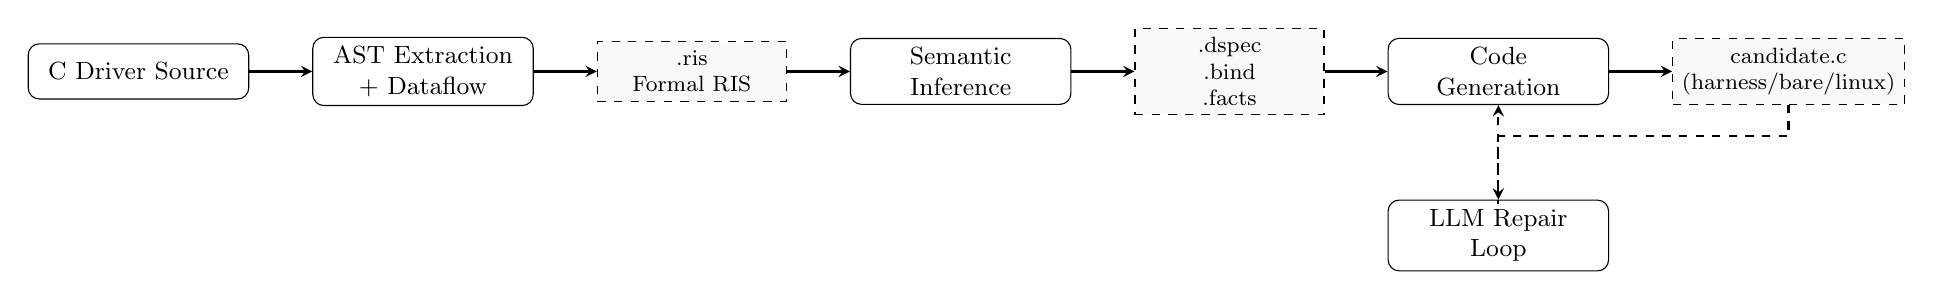
\begin{tikzpicture}[
  node distance=0.8cm,
  block/.style={rectangle, draw, rounded corners, minimum width=2.8cm, minimum height=0.7cm, align=center, font=\small},
  arrow/.style={->, >=stealth, thick},
  artifact/.style={rectangle, draw, dashed, fill=gray!5, minimum width=2.4cm, minimum height=0.6cm, align=center, font=\footnotesize},
]

\node[block] (src) {C Driver Source};
\node[block, right=of src] (extract) {AST Extraction\\+ Dataflow};
\node[artifact, right=of extract] (ris) {.ris\\Formal RIS};
\node[block, right=of ris] (infer) {Semantic\\Inference};
\node[artifact, right=of infer] (dspec) {.dspec\\.bind\\.facts};
\node[block, right=of dspec] (gen) {Code\\Generation};
\node[artifact, right=of gen] (code) {candidate.c\\(harness/bare/linux)};

\draw[arrow] (src) -- (extract);
\draw[arrow] (extract) -- (ris);
\draw[arrow] (ris) -- (infer);
\draw[arrow] (infer) -- (dspec);
\draw[arrow] (dspec) -- (gen);
\draw[arrow] (gen) -- (code);

\node[block, below=1.2cm of gen] (llm) {LLM Repair\\Loop};
\draw[arrow, dashed] (code.south) -- ++(0,-0.4) -| (llm);
\draw[arrow, dashed] (llm) -- ++(0,0.4) -| (gen.south);

\end{tikzpicture}%
}
\caption{\reharness pipeline. C source is parsed via libclang to extract formal RIS; semantic inference enriches RIS into backend-independent specs; code generation targets multiple backends; a dashed LLM repair loop patches candidates under verification feedback.}
\label{fig:arch}
\end{figure}

\textbf{Stage 1: RIS Extraction.} The extraction stage parses C source with libclang, builds a macro offset table from preprocessing records, identifies driver entry points, and performs per-function flow-sensitive dataflow analysis. The output is a formal \rislang specification recording every register read, write, and RMW operation with symbolic register names, branch guards, and width annotations.

\textbf{Stage 2: Semantic Inference.} The inference stage enriches raw \rislang modules with backend-independent semantics. It infers function roles from callback table registrations (e.g., \texttt{.irq\_ack = ftgpio\_ack\_irq} $\rightarrow$ \texttt{interrupt\_ack}), abstracts C parameter types to formal types (e.g., \texttt{struct irq\_data *} $\rightarrow$ \texttt{LogicalIRQ}), binds MMIO bases to device state, and derives effects and Hoare-style contracts from role semantics. The result is a \texttt{FunctionSpec} per driver function, composed into a \texttt{DeviceSpec} with state, resources, register map, and invariants.

\textbf{Stage 3: Code Generation.} The generation stage consumes the formal specs and backend-specific binding files to produce driver code for three targets: (1) a userspace harness with fake MMIO memory and trace logging for testing, (2) portable bare-metal C for embedded systems, and (3) Linux kernel modules with platform, PCI, GPIO/IRQ, and miscdevice lifecycle glue selected from the inferred device class. When an operation depends on source-private state that is not represented in the formal specification, generation emits an explicit unsupported marker and neutral code instead of inventing behavior.

\textbf{Stage 4: LLM-Assisted Synthesis.} When the deterministic backend cannot fully reconstruct source-private state or complex subsystem semantics, \reharness assembles a structured bundle of \rislang, device spec, backend binding, source facts, and a deterministic candidate. It then enters a closed loop: compile/static/trace verification yields structured feedback, which is fed to an LLM as a repair prompt. The LLM patches the candidate, and the loop repeats until the candidate passes all checks or the iteration budget is exhausted.

\section{Formal RIS Language}

The core output of \reharness is the \rislang (Register Interaction Sequence) specification language. \rislang is designed to be both human-readable and machine-parseable, with a formal grammar supporting the full vocabulary of MMIO operations found in real drivers.

\subsection{Grammar}

\begin{lstlisting}[language=ris]
driver <name> v<version> {
  module <function_name> {
    <var> := R(<width>, <addr>) [-- <intent>]
    W(<width>, <addr>) = <expr> [-- <intent>]
    RMW(<width>, <addr>) = <transform> [-- <intent>]
    IF <guard> { <ops> } [ELSE { <ops> }]
    LOOP <count> { <ops> }
    DELAY(<cycles>)
  }
}
\end{lstlisting}

Each \texttt{module} corresponds to a driver function (a framework callback or helper). Operations within a module are ordered as they appear in source, preserving the program's execution sequence.

\subsection{Operations}

\textbf{Read (\texttt{R})}: A register read with a bound variable for later use. Width is one of \texttt{B1}, \texttt{B2}, \texttt{B4}, \texttt{B8} (inferred from the MMIO call's suffix: \texttt{readl} $\rightarrow$ B4, \texttt{readw} $\rightarrow$ B2, etc.). The address is resolved to one of three forms:

\begin{itemize}
\item \textbf{Symbolic:} \texttt{g->base.GPIO\_INT\_EN}---a known base expression plus a resolved register macro.
\item \textbf{Fixed:} \texttt{0x20}---a literal offset with no macro resolution.
\item \textbf{Computed:} \texttt{[g->base + idx]}---a dynamic address expression that could not be statically resolved.
\end{itemize}

\textbf{Write (\texttt{W})}: A register write with an expression value, which may be a constant, a variable, or a compound expression in the \texttt{Expr} algebra.

\textbf{Read-Modify-Write (\texttt{RMW})}: Detected when a \texttt{writel} value is the result of modifying a \texttt{readl} return from the same address. This is a critical pattern for interrupt mask/unmask operations, where a single bit must be toggled without disturbing others.

\textbf{Conditional (\texttt{IF})}: Branch conditions extracted from \texttt{if/else} statements and attached to operations within each branch. A predicate stack retains nested guards and distinguishes then paths from negated else paths.

\textbf{Loop (\texttt{LOOP})}: Iteration constructs from \texttt{for/while} loops, annotated with a count expression when statically derivable.

\textbf{Delay (\texttt{DELAY})}: Timing operations (\texttt{mdelay}, \texttt{udelay}, \texttt{msleep}) converted to nanosecond-equivalent counts.

\subsection{Expression Algebra}

Values and guards in \rislang are represented in an algebraic expression language:

\begin{center}
\resizebox{\columnwidth}{!}{%
\begin{tabular}{ll}
\texttt{Expr} & $::=$ \texttt{Const($n$)} $|$ \texttt{Var($x$)}
$|$ \texttt{BinOp\{op, left, right\}} $|$ \texttt{Ite\{guard, then, else\}} $|$ \texttt{Bits\{hi, lo, expr\}} $|$ \texttt{Top} \\
\end{tabular}%
}
\end{center}

\texttt{BinOp} supports arithmetic, bitwise, relational, and logical operators. \texttt{Ite} represents a path-conditioned value and is emitted as a C conditional expression by all backends. The \texttt{Top} sentinel represents values that could not be statically resolved.

Example expressions:
\begin{lstlisting}[breaklines=true]
0x1 << irqd_to_hwirq(d)
  -> BinOp{Shl, Const(1), Var("irqd_to_hwirq(d)")}
0x0 ^ 0xffffffff
  -> BinOp{BitXor, Const(0), Const(0xffffffff)}
\end{lstlisting}

\subsection{Example}

Listing~\ref{lst:ris_example} shows the extracted \rislang for the \texttt{gpio-ftgpio010} driver, a Faraday FTGPIO010 GPIO controller. Each module corresponds to a callback registered through the Linux \texttt{irq\_chip} and \texttt{gpio\_chip} framework tables.

\begin{lstlisting}[language=ris,label={lst:ris_example},caption={Extracted \rislang specification for gpio-ftgpio010 (7 modules, 22 ops)}]
driver gpio-ftgpio010 v0.1.0 {
  module ftgpio_gpio_ack_irq {
    W(B4, g->base.GPIO_INT_CLR) = (0x1 << irqd_to_hwirq(d))
         -- Interrupt
  }
  module ftgpio_gpio_mask_irq {
    val := R(B4, g->base.GPIO_INT_EN) -- Interrupt
    RMW(B4, g->base.GPIO_INT_EN) = val -- Interrupt
  }
  module ftgpio_gpio_unmask_irq {
    val := R(B4, g->base.GPIO_INT_EN) -- Interrupt
    RMW(B4, g->base.GPIO_INT_EN) = val -- Interrupt
  }
  module ftgpio_gpio_set_irq_type {
    reg_type  := R(B4, g->base.GPIO_INT_TYPE) -- Interrupt
    reg_level := R(B4, g->base.GPIO_INT_LEVEL) -- Interrupt
    reg_both  := R(B4, g->base.GPIO_INT_BOTH_EDGE) -- Interrupt
    RMW(B4, g->base.GPIO_INT_TYPE) = reg_type
    RMW(B4, g->base.GPIO_INT_LEVEL) = reg_level
    RMW(B4, g->base.GPIO_INT_BOTH_EDGE) = reg_both
  }
  module ftgpio_gpio_irq_handler {
    stat := R(B4, g->base.GPIO_INT_STAT_RAW) -- Interrupt
  }
  module ftgpio_gpio_set_config {
    val := R(B4, g->base.GPIO_DEBOUNCE_PRESCALE) -- Config
    IF (val == deb_div) {
      val := R(B4, g->base.GPIO_DEBOUNCE_EN) -- Config
      RMW(B4, g->base.GPIO_DEBOUNCE_EN) = val -- Config
    }
    ...
  }
  module ftgpio_gpio_probe {
    W(B4, g->base.GPIO_INT_EN)  = 0x0 -- Init
    W(B4, g->base.GPIO_INT_MASK) = 0x0 -- Init
    ...
  }
}
\end{lstlisting}

All 22 register operations in this driver are resolved to symbolic addresses (100\% symbolic rate). The mask/unmask callbacks correctly exhibit RMW patterns (read the current interrupt enable mask, modify it, write it back). The \texttt{set\_config} module preserves the conditional guard \texttt{(val == deb\_div)} around the debounce-enable RMW.

\section{RIS Extraction via AST Analysis}

\subsection{Translation Unit Parsing}

\reharness uses libclang to parse each C source file as an unsaved translation unit, enabling preservation of macro expansion records. The parser operates in tolerant mode, continuing past syntax errors that would halt a regular compiler (essential for drivers that depend on kernel headers not available in the analysis environment). Parsing yields a complete AST cursor tree plus a \texttt{MacroTable} built from preprocessing records.

The \texttt{MacroTable} maps every \texttt{\#define} in the translation unit to its expanded value. For integer-valued register macros (e.g., \texttt{\#define GPIO\_INT\_EN 0x20}), we record the numeric offset. This table is the critical data structure that enables symbolic address resolution: when the dataflow analyzer encounters a reference to \texttt{GPIO\_INT\_EN} in an address expression, it can resolve it to 0x20 and pair it with the base pointer to produce a \texttt{Symbolic} address.

\subsection{Function Identification and Callback Detection}

Target functions are identified by traversing the AST for function definitions whose source location is in the target file. Each function is modeled as a \texttt{Func} object with its name, parameter list, return type, and cursor.

Callback entries are recovered from designated initializers and member assignments, while tracking the enclosing structure type. The field and structure are matched against a role table (\texttt{FIELD\_ROLE}); for example, \texttt{.irq\_ack = ftgpio\_gpio\_ack\_irq} becomes the full binding \texttt{irq\_chip.irq\_ack} with role \texttt{interrupt\_ack}. Functions without a recognized framework binding are classified as helpers and may be inlined into callers.

\subsection{Flow-Sensitive Dataflow and Taint Tracking}

The core of the extraction is a per-function flow-sensitive dataflow analysis. For each function, we walk its call sites in source order, maintaining an abstract store mapping variable names to abstract values (\texttt{AbsVal}) drawn from a finite domain:

\begin{center}
\begin{tabular}{ll}
\texttt{AbsVal} & $::=$ \texttt{BasePtr($b$)} $|$ \texttt{Offset($b$, $n$, $r$)} $|$
\texttt{ReadTaint($a$, $r$)} $|$ \\
& \quad\;\; \texttt{Const($n$)} $|$ \texttt{SymExpr($e$)} $|$ \texttt{Top} \\
\end{tabular}
\end{center}

\textbf{Taint sources}: \texttt{ioremap} and its direct or devres-managed variants are recognized as MMIO base-pointer sources. The variable receiving the mapping is bound to \texttt{BasePtr}.

\textbf{Address resolution}: When an MMIO read/write call is encountered, its address argument is symbolically evaluated against the abstract store and macro table. The evaluation resolves \texttt{base + REG} expressions by combining the \texttt{BasePtr} for the pointer variable with the \texttt{Offset} value from the macro table, producing a \texttt{Symbolic} address carrying both the device context and the register name.

\textbf{Read taint}: The return value of a \texttt{readl} call is bound to \texttt{ReadTaint(addr)}, recording which address was read. When a subsequent \texttt{writel} uses a value that evaluates to a \texttt{ReadTaint} of the \textit{same} address, \reharness detects a read-modify-write pattern and emits an \texttt{RMW} operation instead of separate read and write.

\textbf{Expression evaluation}: A recursive descent evaluator handles arithmetic (\texttt{+}, \texttt{-}, \texttt{<<}, \texttt{>>}), bitwise (\texttt{|}, \texttt{\&}, \texttt{\^{}}), and unary (\texttt{\~{}}) operations over abstract values. Constant folding is applied where both operands are \texttt{Const}; otherwise, the expression is captured as a \texttt{SymExpr} or \texttt{BinOp} for the formal \rislang output.

\subsection{Wrapper Function Inlining}

When a call site references a function defined in the same translation unit that is not a framework primitive (not in \texttt{FRAMEWORK\_FNS}), \reharness checks whether that function has been previously extracted. If so, its operations are inlined at the call site, with the call site's branch condition applied to each inlined operation. Inlining depth is bounded (default 3) to prevent infinite recursion through mutually recursive helpers.

This is a lightweight form of inter-procedural analysis: we do not perform full context-sensitive summary computation, but the bounded-depth inlining is sufficient to expose MMIO operations hidden in common wrapper patterns such as \texttt{gpio\_setbit}, \texttt{reg\_read}, and \texttt{reg\_write}.

\subsection{Intent Annotation}

Each operation is annotated with an \emph{intent} string derived from the resolved register macro name. We classify register names using keyword matching: registers containing ``INT'' or ``IRQ'' are assigned intent \texttt{Interrupt}; ``CLK'' or ``PLL'' yield \texttt{Clock}; ``CONFIG'' or ``CTRL'' yield \texttt{Config}; ``STAT'' yields \texttt{Status}; and so on. This lightweight heuristic provides human-readable context without requiring deep semantic analysis.

\section{Semantic Inference}

The raw \rislang captures what registers are accessed and how, but does not explain \emph{why}---what role each function plays in the driver, what effects it has on device state, and what contracts it must satisfy. \reharness enriches \rislang modules with backend-independent semantics through three layers of inference.

\subsection{Function Specification (FunctionSpec)}

A \texttt{FunctionSpec} is a tuple:

\[
(\text{Signature}, \text{Role}, \text{Context}, \text{Binds}, \text{Requires}, \text{Ensures}, \text{Effects}, \text{RISRef})
\]

\textbf{Role inference} is the critical step. \reharness prioritizes callback table bindings over function-name heuristics. When a callback table field is recognized (e.g., \texttt{.irq\_ack} in an \texttt{irq\_chip} structure), the corresponding role (\texttt{interrupt\_ack}) and execution context (\texttt{irq}) are assigned deterministically. Our \texttt{FIELD\_ROLE} table covers 35+ standard Linux callback fields across \texttt{irq\_chip}, \texttt{platform\_driver}, \texttt{virtio\_config\_ops}, \texttt{gpio\_chip}, and \texttt{dev\_pm\_ops}. For functions not appearing in any callback table, a fallback heuristic matches function name substrings to roles (e.g., \texttt{*\_ack\_irq} $\rightarrow$ \texttt{interrupt\_ack}).

\textbf{Signature abstraction} maps C parameter types to abstract formal types: \texttt{struct irq\_data *} $\rightarrow$ \texttt{LogicalIRQ}, \texttt{struct platform\_device *} $\rightarrow$ \texttt{DeviceState}, integer types $\rightarrow$ \texttt{UInt}, \texttt{void} $\rightarrow$ \texttt{Void}. This abstraction is essential for backend independence: the same \texttt{DeviceSpec} can target Linux, bare-metal, and harness backends without referencing Linux-specific types.

\textbf{State binding} identifies the MMIO base expression used by the function (e.g., \texttt{g->base}) and binds it to a formal \texttt{dev.base} path. The binding is discovered by scanning the address expressions of the function's \rislang operations for member-access patterns.

\textbf{Effects} are derived from two sources: (1) for each symbolic register written by the function, a \texttt{writes\_register(REG)} effect is emitted; (2) from the function's role, a semantic event effect is derived (e.g., \texttt{interrupt\_ack} $\rightarrow$ \texttt{clears\_interrupt(line)}).

\textbf{Requires/Ensures} are Hoare-style pre- and postconditions derived from role semantics. For example, an \texttt{interrupt\_ack} function requires nothing and ensures \texttt{interrupt\_pending[line] == false}; a \texttt{probe} function requires \texttt{resources\_available} and ensures \texttt{device\_state == READY}.

\subsection{Device Specification (DeviceSpec)}

A \texttt{DeviceSpec} composes multiple \texttt{FunctionSpec} instances into a device-level model:

\[
(\text{State}, \text{Resources}, \text{Registers}, \text{Functions}, \text{Invariants}, \text{Class})
\]

\textbf{Device class} is inferred from the driver name (e.g., \texttt{gpio-ftgpio010} $\rightarrow$ \texttt{gpio\_controller}, \texttt{virtio\_mmio} $\rightarrow$ \texttt{virtio\_mmio}).

\textbf{State} is inferred from the functions' needs: every device gets an \texttt{MmioBase} state field; if any function has a clock-related role or the source mentions \texttt{clk}, a \texttt{Clock} field is added; if any function has an interrupt-related role, a \texttt{num\_irqs: UInt} field is added.

\textbf{Resources} are derived from the state fields: an \texttt{MmioResource} bound to \texttt{base}, plus \texttt{ClockResource} and \texttt{IrqResource} as needed.

\textbf{Registers} are collected from the \rislang's \texttt{register\_map}, which contains every symbolic register actually accessed by the driver (not every register the hardware defines, only the ones the driver touches).

\textbf{Invariants} are generated as minimal safety properties: for interrupt-capable devices, the invariant \texttt{forall line: UInt. line < num\_irqs -> valid\_interrupt\_line(line)} is asserted.

\subsection{Backend Binding (.bind)}

A \texttt{BindSpec} maps abstract concepts from the \texttt{DeviceSpec} to concrete backend APIs:

\begin{itemize}
\item \textbf{Type maps:} \texttt{DeviceState $\rightarrow$ "struct ftgpio\_gpio"}, \texttt{MmioBase $\rightarrow$ "void \_\_iomem *"} (Linux) or \texttt{uintptr\_t} (bare-metal).
\item \textbf{Callback maps:} \texttt{irq\_chip.irq\_ack = ftgpio\_gpio\_ack\_irq}.
\item \textbf{Primitive maps:} \texttt{MmioRead(B4) $\rightarrow$ "readl"} (Linux) or \texttt{mmio\_read32} (bare-metal).
\item \textbf{State maps:} \texttt{dev.base $\rightarrow$ "g->base"}.
\item \textbf{Export maps:} \texttt{interrupt\_ack as "ftgpio\_ack\_irq"} (bare-metal).
\end{itemize}

Default bindings are generated per backend, but can be customized to support non-standard APIs or naming conventions.

\subsection{Source Facts (.facts)}

For LLM-assisted synthesis, \reharness extracts \emph{source facts}---information that aids reconstruction but should not pollute the backend-independent formal spec:

\begin{itemize}
\item \textbf{Includes:} \texttt{<linux/gpio/driver.h>}, \texttt{<linux/platform\_device.h>}.
\item \textbf{Struct definitions:} \texttt{ftgpio\_gpio} with fields \texttt{base: void \_\_iomem *}, \texttt{clk: struct clk *}.
\item \textbf{Constants:} Non-register macros with integer values (flags, status codes, bit masks).
\item \textbf{Callback tables:} \texttt{irq\_chip.irq\_ack = ftgpio\_gpio\_ack\_irq}, etc.
\item \textbf{Resources:} Acquisition calls (\texttt{devm\_platform\_ioremap\_resource}) with bind targets.
\item \textbf{Error paths:} Return codes found in the source (\texttt{-ENOMEM}, \texttt{-ENODEV}, \texttt{PTR\_ERR}).
\item \textbf{Helper calls:} Notable subsystem functions (\texttt{devm\_gpiochip\_add\_data}, \texttt{bgpio\_init}).
\end{itemize}

\section{Code Generation}

\reharness includes a multi-backend code generator that consumes \texttt{(RIS, DeviceSpec, BindSpec)} to produce compilable driver code. Three deterministic backends are provided; a fourth backend uses LLM-assisted synthesis for complex targets.

\subsection{Userspace Harness Backend}

The harness backend generates a self-contained C program that emulates MMIO through a fixed-size memory buffer (\texttt{uint32\_t mmio\_mem[4096]}). Reads and writes are routed through wrapper functions (\texttt{harness\_read32}, \texttt{harness\_write32}) that log every access with a trace line:

\begin{lstlisting}
[trace 0] W 0x20 = 0x00000000  ; GPIO_INT_EN
[trace 1] W 0x30 = 0xffffffff  ; GPIO_INT_CLR
\end{lstlisting}

The harness includes the device state struct, register constants derived from the register map, RIS-backed function bodies (using the backend binding's primitive and state maps), and unit-test scaffolding. The entire harness compiles with a standard C compiler (\texttt{cc -Wall}) and produces a binary that can be executed and traced.

\subsection{Bare-Metal Backend}

The bare-metal backend generates portable C targeting freestanding environments. Instead of Linux kernel types, it uses standard integer types (\texttt{uintptr\_t}, \texttt{uint32\_t}) and portable MMIO primitives (\texttt{mmio\_read32}, \texttt{mmio\_write32}). The generated code includes the device state struct, init/reset/IRQ helper functions, and no framework glue. It compiles with \texttt{cc -ffreestanding -c}.

\subsection{Linux Backend}

The Linux backend generates buildable kernel modules with \texttt{struct device\_state}, \texttt{probe/remove} functions, framework ops tables, and RIS-backed callback bodies using proper Linux MMIO primitives (\texttt{readl}, \texttt{writel}). It provides deterministic resource lifecycles for platform MMIO devices (devres mapping, optional clocks, GPIO/IRQ registration, and OF matching), PCI MMIO devices (enable/request/map/unmap/release and PCI IDs), and QEMU edu (miscdevice \texttt{open/read/write} operations that expose the MMIO oracle). Unsupported source-private state is neutralized only to keep the result buildable and is accompanied by a \texttt{REHARNESS\_UNSUPPORTED} marker that prevents strict-readiness claims.

\subsection{LLM-Assisted Synthesis Loop}

When deterministic generation is insufficient---for example, when the Linux backend cannot fully reconstruct the probe/resource lifecycle or subsystem-specific registration glue---\reharness enters a closed-loop LLM-assisted synthesis mode (Figure~\ref{fig:arch}, dashed path).

The synthesis module assembles a structured input bundle: \texttt{device.ris}, \texttt{device.dspec}, \texttt{device.<backend>.bind}, \texttt{device.facts}, \texttt{device.scaffold.c}, and two guiding documents (\texttt{constraints.md} and \texttt{verification.md}). The scaffold is the output of the deterministic generator.

The repair loop operates as follows:

\begin{enumerate}
\item \textbf{Compile:} The candidate is compiled with strict warnings for the target backend.
\item \textbf{Static checks:} Every \rislang reference resolves to a module; every symbolic register is in the register map; every callback entry has a table binding; no TODOs remain.
\item \textbf{Trace check} (harness only): The generated harness is executed and its MMIO trace is compared to the expected trace derived from the \rislang specification.
\item \textbf{Repair:} If any check fails, structured feedback is formatted and sent to an LLM along with the current candidate. The LLM is instructed to produce a patched C candidate that satisfies all constraints.
\item \textbf{Repeat:} Steps 1--4 iterate until the candidate is accepted or the iteration budget (default 3) is exhausted.
\end{enumerate}

The LLM is a pluggable component implemented through the Pi agent SDK; it is not required by the deterministic evaluation. The reproducible matrix and the two QEMU experiments reported below invoke only the AST extractor and deterministic generators. LLM-assisted runs are evaluated separately because model and endpoint nondeterminism would otherwise confound artifact reproduction.

\section{Evaluation}

We evaluate \reharness on \EvalDrivers{} versioned Linux driver sources covering GPIO, clock/PLL, AHCI, SDHCI, virtio-MMIO, a framebuffer raster engine, and QEMU edu. The evaluation addresses five research questions:

\begin{itemize}
\item \textbf{RQ1 (Precision):} What fraction of register accesses are resolved to symbolic addresses?
\item \textbf{RQ2 (Completeness):} How many RMW patterns and branch conditions are detected?
\item \textbf{RQ3 (Generation):} Do the generated harness, bare-metal, and Linux targets compile?
\item \textbf{RQ4 (Comparison):} How does \reharness compare to the regex-based baseline?
\item \textbf{RQ5 (Runtime):} Do deterministically generated drivers preserve register behavior on real QEMU devices?
\end{itemize}

\subsection{Experimental Setup}

All experiments were run on a Linux machine with an AMD 9950X processor and 64~GB RAM, using Python 3, libclang 18, and the pinned Linux submodule commit recorded in \path{experiments/results/matrix.json}. The kernel configuration (including \texttt{CONFIG\_COMMON\_CLK=y}), QEMU scripts, driver corpus, and source hashes are versioned with the artifact. The complete 19-driver extraction/generation/Kbuild matrix takes approximately 89.0 seconds (4.68 seconds per driver on average) after the experiment kernel has been built.

\subsection{Extraction Coverage (RQ1, RQ2)}

Table~\ref{tab:extraction} is generated directly from the machine-readable experiment result and summarizes extraction across all \EvalDrivers{} drivers.

\begin{table}[t]
\centering
\caption{Extraction statistics across \EvalDrivers{} test drivers. Sym, Fixed, and Comp are distinct address classes.}
\label{tab:extraction}
\resizebox{\columnwidth}{!}{\ExtractionResultsTable}
\end{table}

\textbf{Key finding:} \reharness preserves three address classes instead of forcing all accesses into a symbolic-name category. Of the address-bearing operations, \EvalSymbolicPct{} are symbolic, while fixed offsets and runtime-computed addresses remain explicit. This corrects an earlier evaluation mistake that conflated ``resolved'' with ``symbolic.'' The distinction matters: indexed virtio configuration accesses and banked GPIO registers are representable but cannot honestly be assigned one static register name.

The \EvalRMW{} detected RMW patterns are concentrated in interrupt mask/unmask callbacks and configuration functions. Straight-line mutations such as \texttt{val \&= \~BIT(line)} are retained as transforms. Branch-dependent switch updates are represented as nested \texttt{Ite} expressions, with every branch applied independently to the original read value rather than incorrectly concatenated.

The \EvalConditions{} recorded branch conditions occur primarily in configuration and probe functions that check device state before modifying registers.

\subsection{Multi-Source Driver Scaling}

The initial corpus treats one C translation unit as one extraction target. To evaluate realistic module scale, we added versioned manifests for Kbuild modules composed from four or more C files. Each manifest is checked against the pinned Linux module's actual \texttt{*-y} object list; the files are not unrelated drivers grouped after the fact. The extractor builds every translation unit with its own preprocessing context, merges macros and source facts, and iteratively propagates MMIO summaries across file boundaries before constructing one combined RIS and DeviceSpec.

\begin{table}[t]
\centering
\caption{Real multi-source Linux driver modules. TUs are C translation units; H/B/L reports harness, bare-metal, and Linux compilation.}
\label{tab:multisource}
\resizebox{\columnwidth}{!}{\MultiSourceResultsTable}
\end{table}

Table~\ref{tab:multisource} covers \MultiSourceTUs{} translation units and \MultiSourceLines{} source lines, yielding \MultiSourceOps{} operations, \MultiSourceRMW{} RMW patterns, and \MultiSourceRegisters{} mapped registers. C67X00 demonstrates cross-file propagation from its low-level HPI implementation into probe and IRQ entry points. ASPEED vHub increases the scale to five files and preserves 154 operations across endpoint, hub, interrupt, and probe paths. All generated backends compile for both modules, while strict readiness remains conservative because USB subsystem callback/state models are not yet complete.

\subsection{Generation Readiness (RQ3)}

Table~\ref{tab:readiness} separates compilation from strict semantic readiness. A generated file can compile while still carrying an explicit unsupported state-binding marker.

\begin{table}[t]
\centering
\caption{Generation readiness scores per driver.}
\label{tab:readiness}
\resizebox{\columnwidth}{!}{\ReadinessResultsTable}
\end{table}

Harness, bare-metal, and Linux outputs compile for \EvalDrivers{}/\EvalDrivers{} drivers. In contrast, only \LinuxReadyCount{}/\EvalDrivers{} currently satisfies strict Linux readiness, and \LLMReadyCount{}/\EvalDrivers{} have sufficient structured context for assisted synthesis. This is intentional: unknown transforms, unsafe computed addresses, target-source clang errors, and normalized source-private state block readiness even when code can be compiled. Lowerable computed expressions, such as PL061's banked GPIO address, are generated exactly and do not block readiness. The mean RIS quality is \EvalMeanRIS{}.

\subsection{Comparison to Regex Baseline (RQ4)}

We compare \reharness against \texttt{driver-harness}, a regex-based tool that served as \reharness's predecessor and baseline. The comparison focuses on the four failure patterns identified in Section~\ref{sec:motivation}.

\begin{table}[t]
\centering
\caption{Comparison of \reharness vs. regex baseline on four key patterns.}
\label{tab:comparison}
\resizebox{\columnwidth}{!}{%
\begin{tabular}{lcc}
\hline
\textbf{Pattern} & \textbf{Regex Baseline} & \textbf{\reharness} \\
\hline
Macro register offsets & 0\% resolved & Constants recovered from AST \\
Wrapper function inlining & MMIO lost & Inlined (depth $\le$ 3) \\
Branch conditions & Always \texttt{None} & \EvalConditions{} conditions recorded \\
Arithmetic addresses & Not supported & Symbolic/fixed/computed preserved \\
RMW detection & Not supported & \EvalRMW{} RMW patterns \\
\hline
\end{tabular}%
}
\end{table}

The regex baseline resolves 0\% of macro-defined register offsets because it cannot evaluate preprocessor constants. It misses MMIO operations inside wrapper functions, reports \texttt{None} for branch conditions, and cannot classify arithmetic address expressions. \reharness addresses these patterns through AST-level analysis while preserving the distinction between \EvalSymbolic{} symbolic, \EvalFixed{} fixed, and \EvalComputed{} computed-address operations. It therefore avoids both the baseline's lost accesses and the unsound claim that every representable address has one static symbolic name.

\subsection{Case Study: gpio-ftgpio010}

We examine the FTGPIO010 GPIO controller driver in detail. This driver registers 7 callback functions across two Linux framework tables (\texttt{irq\_chip} and \texttt{gpio\_chip}). The driver defines 13 register macros via \texttt{\#define}, of which 9 are actually accessed by the driver code.

\reharness correctly extracts all 22 register operations across 7 modules, resolves all 9 accessed registers to their macro names and numeric offsets, detects 7 RMW patterns (in \texttt{mask\_irq}, \texttt{unmask\_irq}, \texttt{set\_irq\_type}, and \texttt{set\_config}), and records 1 explicit branch condition in \texttt{set\_config}. All 7 functions receive semantic roles and full enclosing-structure callback bindings, including \texttt{gpio\_chip.set\_config} and \texttt{gpio\_irq\_chip.parent\_handler}. The three switch-dependent RMW operations in \texttt{set\_irq\_type} are represented as nested \texttt{Ite} transforms covering edge-both, rising, falling, level-high, and level-low cases; none contains \texttt{Top}.

The generated userspace harness compiles with \texttt{cc -Wall}, the bare-metal C compiles with \texttt{cc -ffreestanding -c}, and the Linux output builds through the pinned kernel's Kbuild interface. In QEMU, a versioned platform-device registrar triggers the generated driver's probe path. Its instrumented trace matches the RIS-derived oracle with \FTQEMUModuleCoverage{} module, \FTQEMUOpCoverage{} operation, and \FTQEMURegisterCoverage{} register coverage (\texttt{\FTQEMUOracle}).

\subsection{Deterministic Runtime Validation (RQ5)}

The runtime experiments are executed by \path{verification/run_qemu_experiments.sh} and recorded in \path{experiments/results/qemu.json}; neither experiment invokes an LLM. For QEMU edu, the deterministic PCI backend generates a miscdevice that provides positional reads and writes over the mapped BAR. The guest exerciser validates the device ID at offset 0x00, the complemented live-check value at 0x04, and the factorial result at 0x08. All value-level checks pass (\texttt{\EduQEMUOracle}).

For gpio-ftgpio010, the experiment registers a platform device, loads the instrumented deterministic module, and compares the emitted MMIO offsets and order against the extracted probe RIS. The oracle passes (\texttt{\FTQEMUOracle}) with \FTQEMUModuleCoverage{} module coverage, \FTQEMUOpCoverage{} operation coverage, and \FTQEMURegisterCoverage{} register coverage. These experiments validate two complementary properties: concrete read/write values on a modeled PCI device and access order/offset preservation for a Linux platform-driver probe path.

\section{Related Work}

\subsection{Driver Analysis and Extraction}

\textbf{C-to-Rust translation.} The C2Rust project~\cite{emrath2021c2rust} performs syntactic translation from C to unsafe Rust, leaving the insertion of safe ownership and borrowing annotations to subsequent tools. \&inator~\cite{andinator2026} addresses the interface translation problem by modeling Rust type selection as an SMT constraint satisfaction problem over type fragments, pointer transformation graphs, and NLL borrowing constraints. \reharness is complementary: it extracts formal register-level behavior that can guide the semantic preservation constraints in C2Rust-style translators.

\textbf{Static driver analysis.} Tools such as SDV~\cite{ball2006thorough}, Dingo~\cite{ryzhyk2009dingo}, and Termite~\cite{ryzhyk2009termite} perform static analysis on driver source to verify protocol compliance and generate boilerplate. These tools operate at the framework API level (e.g., verifying that \texttt{probe} allocates resources and \texttt{remove} frees them). \reharness operates at a lower level: it extracts the actual register interaction sequences, which capture the hardware protocol rather than the OS framework protocol.

\textbf{Symbolic execution.} KLEE~\cite{cadar2008klee} and S2E~\cite{chipounov2011s2e} perform symbolic execution of driver code to generate test inputs. \reharness's extraction is static rather than dynamic, making it applicable to drivers that cannot be executed in a test environment (e.g., due to missing hardware or kernel infrastructure).

\subsection{Formal Specification and Code Generation}

\textbf{Device driver synthesis.} Termite-2~\cite{ryzhyk2014termite2} synthesizes drivers from formal specifications of device and OS interfaces. The specifications must be written manually in a domain-specific language. \reharness automates the specification extraction step, producing \texttt{DeviceSpec} and \texttt{BindSpec} automatically from existing C source.

\textbf{LLM-based code generation.} Recent work explores using large language models for driver synthesis~\cite{roelofs2023large}. These approaches typically operate on natural language descriptions or source snippets. \reharness's LLM-assisted synthesis module is unique in providing structured formal specifications and verification feedback as input constraints, enabling a repair loop rather than one-shot generation.

\subsection{Intermediate Representations for Drivers}

\textbf{Devicetree and ACPI.} Hardware description standards such as Devicetree and ACPI describe the hardware topology (register base addresses, interrupt lines, clocks) but not the register interaction protocols. \reharness's \rislang and \texttt{DeviceSpec} complement these standards by capturing the behavioral protocol.

\textbf{Haiku and Barrelfish driver models.} The Haiku~\cite{haiku} and Barrelfish~\cite{baumann2009multikernel} operating systems use driver models that separate device logic from OS framework code, similar to \reharness's separation of \texttt{DeviceSpec} (what the device does) from \texttt{BindSpec} (how it connects to an OS). \reharness provides the tooling to extract these specifications from existing Linux drivers.

\section{Discussion and Limitations}
\label{sec:discussion}

\subsection{Current Limitations}

\textbf{Linux subsystem coverage.} \reharness recognizes GPIO and IRQ tables (\texttt{gpio\_chip}, \texttt{irq\_chip}, and \texttt{gpio\_irq\_chip}); bus drivers (\texttt{platform\_driver}, \texttt{pci\_driver}, and \texttt{amba\_driver}); and virtio, clock, power-management, and file-operation tables. Other subsystems, including I2C and SPI, require additional callback and lifecycle models.

\textbf{Dataflow precision.} The flow-sensitive analysis retains branch predicates and merges common switch/if RMW patterns into conditional expressions, but it does not maintain a fully separate abstract store for arbitrary control-flow paths. Complex joins, loops, indirect calls, and unmodeled aggregate state can therefore still exceed the native domain. SVF alias analysis is available as an opt-in mode (\texttt{auto} or \texttt{required}) because its external toolchain and analysis cost would otherwise weaken deterministic reproduction; the default evaluation uses the built-in analysis with alias mode \texttt{off}.

\textbf{Linux backend completeness.} The deterministic Linux backend emits Kbuild-compilable output for \LinuxCompileCount{}/\EvalDrivers{} drivers and implements concrete platform, PCI, GPIO/IRQ, clock, power-management, and edu lifecycles. Compilation is not treated as semantic completion: only \LinuxReadyCount{}/\EvalDrivers{} is strictly ready. Common GPIO, clock, and virtio private fields are represented in the generated device state; subsystem-specific objects that remain unbound are replaced with neutral expressions and explicit unsupported markers. Unknown transforms and unsafe computed addresses likewise block strict readiness.

\textbf{Computed addresses.} \reharness preserves the complete runtime offset expression for indexed register banks and emits it directly when every term is lowerable. Such an access still lacks one static symbolic register name, but it is not inherently unsafe. Expressions containing unknown calls, unbound members, or \texttt{Top} remain explicit readiness blockers.

\textbf{LLM reproducibility.} LLM-assisted synthesis remains useful for candidates with sufficient structured context (\LLMReadyCount{}/\EvalDrivers{} in our readiness metric), but model versions, endpoints, and sampling introduce nondeterminism. For that reason, all headline extraction, compilation, and QEMU results use only deterministic stages; LLM outcomes are not included in the runtime claims.

\textbf{Time complexity.} The libclang parsing step is the dominant cost: parsing a typical Linux driver with full kernel headers takes 10--30 seconds. This is acceptable for batch analysis of individual drivers but would be prohibitive for whole-kernel analysis.

\subsection{Future Work}

\textbf{Additional backends.} The backend-binding architecture is designed for extensibility. We plan to add backends for RTOS targets (FreeRTOS, Zephyr) and verification targets (CBMC, SeaHorn) that consume the same \texttt{DeviceSpec} with different \texttt{BindSpec} files.

\textbf{Stateful RIS modeling.} The current \rislang captures op sequences but not device state transitions. A stateful extension that models register state machines (e.g., finite-state automata over register values) would enable stronger verification, such as checking that the driver never reads a register before it is initialized.

\textbf{Whole-kernel analysis.} Scaling extraction to thousands of kernel drivers requires incremental parsing, caching of macro tables and call graphs, and parallel execution. The modular nature of \reharness (per-driver, per-function extraction) makes this feasible.

\textbf{Integration with safe-language translation.} A natural next step is integrating \reharness with C2Rust-style translators: the extracted \rislang and \texttt{DeviceSpec} can inform the type selection and ownership annotation decisions, particularly for MMIO pointers and interrupt handler contexts.

\section{Conclusion}

We presented \reharness, a pipeline for extracting formal register interaction specifications from C device drivers using libclang AST analysis with flow-sensitive dataflow and taint tracking. \reharness overcomes the four fundamental limitations of regex-based extraction: macro-defined register offsets are resolved via preprocessing records, wrapper functions are inlined through inter-procedural call-graph analysis, branch conditions are recorded through predicate stacking, and arithmetic address expressions are evaluated through symbolic abstract interpretation.

Beyond raw extraction, \reharness infers backend-independent function and device semantics, composes them into a multi-backend code generation framework, and provides an optional closed-loop LLM-assisted synthesis module for complex targets. Across \EvalDrivers{} drivers, it extracts \EvalOps{} operations---\EvalSymbolic{} symbolic, \EvalFixed{} fixed, and \EvalComputed{} computed-address---including \EvalRMW{} RMW patterns and \EvalConditions{} conditions, with a mean RIS quality score of \EvalMeanRIS{}. All three deterministic backends compile for \EvalDrivers{}/\EvalDrivers{} drivers, while the explicit \LinuxReadyCount{}/\EvalDrivers{} strict Linux readiness result prevents compilation from being mistaken for semantic completeness. Value-level and trace-level QEMU oracles pass for the deterministic edu and gpio-ftgpio010 outputs.

\reharness enables formal reasoning about driver behavior at the register level, a capability that has been missing from the driver analysis toolchain. By producing specifications in a formal language rather than ad-hoc formats, it provides a foundation for verification, testing, safe-language translation, and AI-assisted driver synthesis.

\begin{acks}
We thank the anonymous reviewers for their constructive feedback.
\end{acks}

\bibliographystyle{ACM-Reference-Format}
\begin{thebibliography}{99}

\bibitem{chou2001empirical}
A.~Chou, J.~Yang, B.~Chelf, S.~Hallem, and D.~Engler.
\newblock An empirical study of operating systems errors.
\newblock In \emph{Proc. SOSP}, 2001.

\bibitem{swift2003improving}
M.~M.~Swift, B.~N.~Bershad, and H.~M.~Levy.
\newblock Improving the reliability of commodity operating systems.
\newblock In \emph{Proc. SOSP}, 2003.

\bibitem{ball2006thorough}
T.~Ball, E.~Bounimova, B.~Cook, V.~Levin, J.~Lichtenberg, C.~McGarvey, B.~Ondrusek, S.~K.~Rajamani, and A.~Ustuner.
\newblock Thorough static analysis of device drivers.
\newblock In \emph{Proc. EuroSys}, 2006.

\bibitem{ryzhyk2009dingo}
L.~Ryzhyk, P.~Chubb, I.~Kuz, and G.~Heiser.
\newblock Dingo: Taming device drivers.
\newblock In \emph{Proc. EuroSys}, 2009.

\bibitem{kadav2009tolerating}
A.~Kadav, M.~J.~Renzelmann, and M.~M.~Swift.
\newblock Tolerating hardware device failures in software.
\newblock In \emph{Proc. SOSP}, 2009.

\bibitem{witkowski2007automated}
T.~Witkowski, N.~Blanc, D.~Kroening, and G.~Weissenbacher.
\newblock Model checking concurrent Linux device drivers.
\newblock In \emph{Proc. ASE}, 2007.

\bibitem{cadar2008klee}
C.~Cadar, D.~Dunbar, and D.~Engler.
\newblock KLEE: Unassisted and automatic generation of high-coverage tests for complex systems programs.
\newblock In \emph{Proc. OSDI}, 2008.

\bibitem{emrath2021c2rust}
M.~Emrath, P.~V.~D.~Voort, and F.~V.~D.~Lijn.
\newblock C2Rust: Translating C to Rust.
\newblock \emph{https://c2rust.com/}, 2021.

\bibitem{roelofs2023large}
J.~Roelofs, A.~Kadav, and A.~Cidon.
\newblock Large language models as driver synthesizers.
\newblock In \emph{Proc. HotOS}, 2023.

\bibitem{driverharness}
\newblock driver-harness: Regex-based driver register extraction.
\newblock \emph{https://github.com/...}, 2025.

\bibitem{crustbench}
\newblock CRUST-Bench: A benchmark suite for C-to-Rust translation.
\newblock 2024.

\bibitem{ryzhyk2009termite}
L.~Ryzhyk, P.~Chubb, I.~Kuz, E.~L.~Sueur, and G.~Heiser.
\newblock Automatic device driver synthesis with Termite.
\newblock In \emph{Proc. SOSP}, 2009.

\bibitem{ryzhyk2014termite2}
L.~Ryzhyk, A.~Walker, J.~Keys, A.~Legg, A.~Raghunath, M.~Stumm, and M.~Vij.
\newblock User-guided device driver synthesis.
\newblock In \emph{Proc. OSDI}, 2014.

\bibitem{chipounov2011s2e}
V.~Chipounov, V.~Kuznetsov, and G.~Candea.
\newblock S2E: A platform for in-vivo multi-path analysis of software systems.
\newblock In \emph{Proc. ASPLOS}, 2011.

\bibitem{baumann2009multikernel}
A.~Baumann, P.~Barham, P.-E.~Dagand, T.~Harris, R.~Isaacs, S.~Peter, T.~Roscoe, A.~Schüpbach, and A.~Singhania.
\newblock The multikernel: A new OS architecture for scalable multicore systems.
\newblock In \emph{Proc. SOSP}, 2009.

\bibitem{haiku}
\newblock Haiku operating system.
\newblock \emph{https://www.haiku-os.org/}.

\bibitem{andinator2026}
\newblock \&inator: Correct, precise C-to-Rust interface translation.
\newblock In \emph{Proc. PLDI}, 2026.

\end{thebibliography}

\end{document}
